\newpage
\chapter{Simulace fokusační soustavy}

úvod

\section{Koncept einzel lens}

Označení einzel lens se používá pro soustavu typicky tří cylindrických elektrostatických elektrod v řadě za sebou. Soustava slouží k fokusování iontového svazku ve vakuu pomocí specifického elektrického pole, které se běžně vytváří přivedením stejného napětí na krají dvě elektrody a odlišného napětí na prostřední elektrodu. Regulace napětí na prostřední elektrodě je pak dostačující ke kontrolování fokusačních vlastností aparatury, které ovšem celkově závisí i na geometrii elektrod a energii kontrolovaného svazku. Polarita použitého napětí se odvíjí od náboje fokusovaných iontů. V principu je totiž třeba vytvořit takový potenciálový rozdíl mezi elektrodami, aby mezi první a druhou elektrodou ionty překonávaly potenciálový kopec a mezi druhou a třetí elektrodou se vracely k nižšímu potenciálu. Potom vzhledem k zakřivení elektrického pole, které je dané geometrií elektrod, se trajektorie iontů nejprve odchýlý od směru svazku a zpomalý a následně jsou strženy zpět k ose svazku, aby se protly v jednom bodě, je-li poměr mezi napětími krajní a prostřední elektrody vhodně nastavený. To je možné díky tomu, že čím dále je konkrétní iont od osy svazku, tím více na něj působí zakřivení válcově symetrického pole. Energie svazku na výstupu by pak měla být nezměněna právě díky stejným hodnotám napětí na krajních elektrodách.\\

Na Obr. \ref{05schemaEinzelLens} lze vidět schématický nákres čočky, který ilustruje výše popsaný způsob fokusace. Ten jen demonstrovaný též Obr. \ref{05simulaceEinzelLens}, na kterém je výsledek simulace z programu SIMION, který znázorňuje potenciálové hladiny mezi elektrodami v rovině xy. Simulovaná konfigurace z obrázku má následující parametry: válcové elektrody mají průměr $d=35$~mm, krajní elektrody jsou dlouhé $l_o = 2$~mm, prostřední měří, $l_i = 26$~mm, tloušťka stěny válce je $t=1$~mm, napětí na elektrodách jsou $U_o = 5$~kV, $U_i = -18$ kV, energie svazku u zdroje je $E = 20$~keV. Svazek je nastaven tak, aby od zdroje divergoval. Tuto divergenci fokusační soustava zastavuje a směřuje trajektorie do vzdáleného ohniska. Na Obr. \ref{05simulaceEinzelLensPotencial} je pak výše potenciálové hladiny reprezentována třetí souřadnicí, což může pomoci k vytvoření intuitivní představy o průběhu fokusace.\\

\begin{figure}[htbp!]
\centering
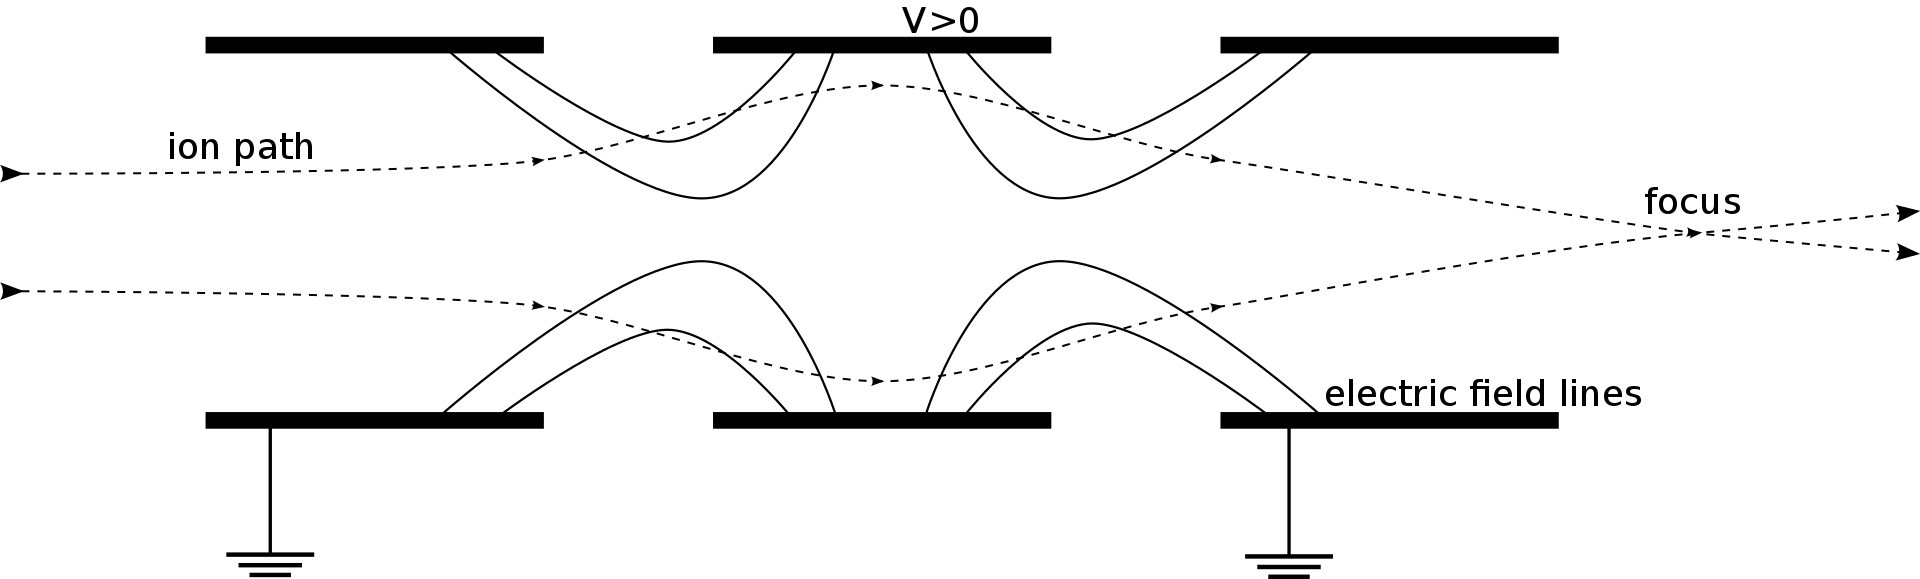
\includegraphics[width = 366 pt]{Figure/05/schema.png}
\caption{Caption.}
\label{05schemaEinzelLens}
\end{figure}

\begin{figure}[htbp!]
\centering
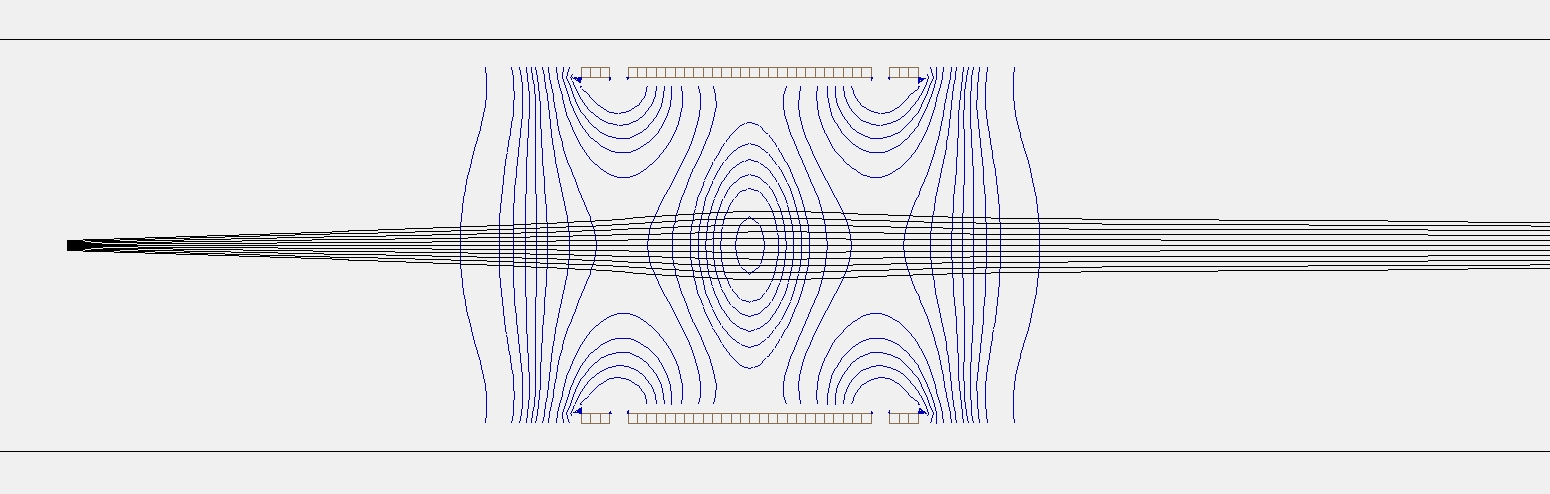
\includegraphics[width = 366 pt]{Figure/05/3a.jpg}
\caption{Caption.}
\label{05simulaceEinzelLens}
\end{figure}

\begin{figure}[htbp!]
\centering
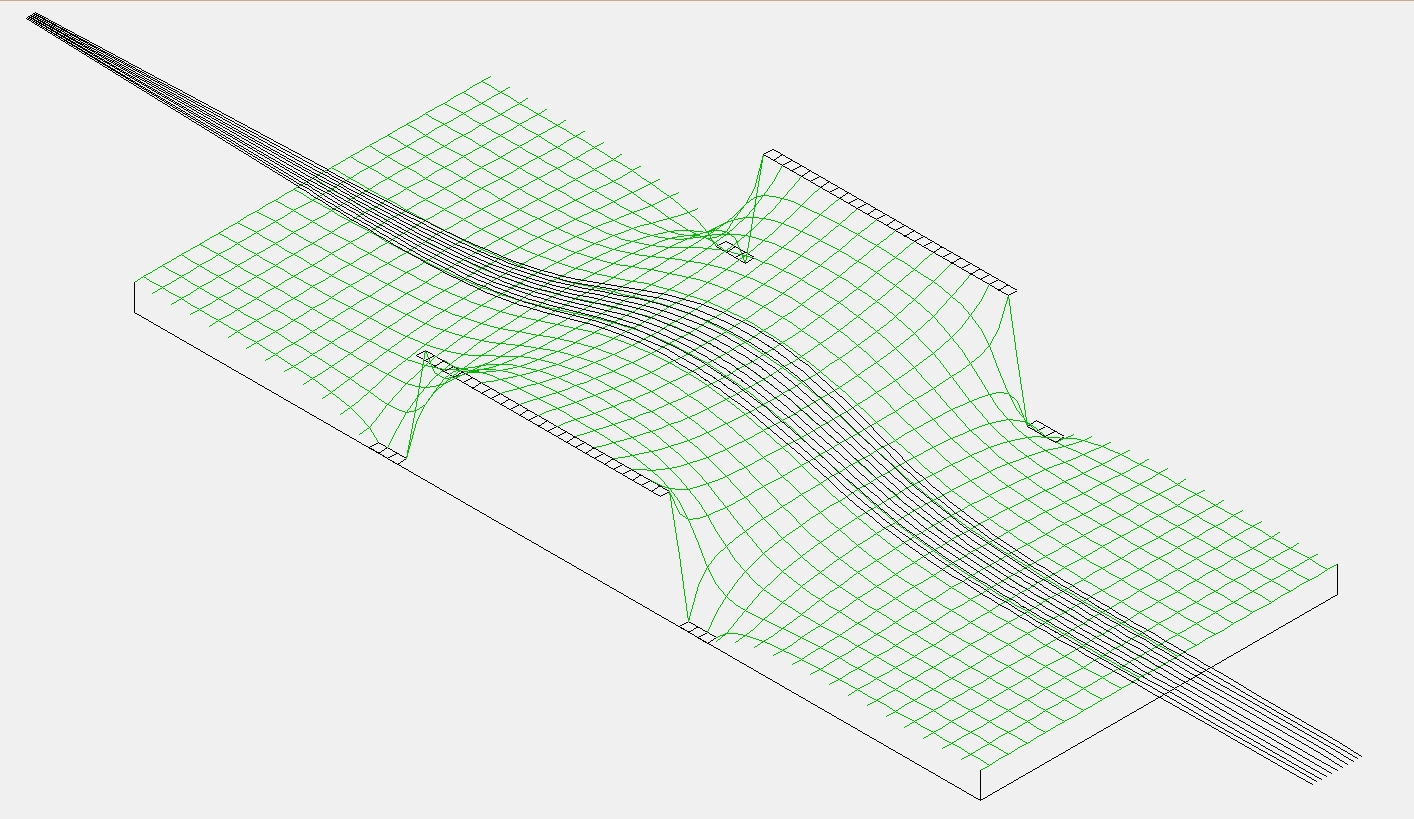
\includegraphics[width = 366 pt]{Figure/05/3b.jpg}
\caption{Caption.}
\label{05simulaceEinzelLensPotencial}
\end{figure}

Podobnou konfiguraci bylo původně v plánu použít k regulaci elektronového svazku z děla CRT obrazovky. Vzhledem k tomu, že se toto dělo nepodařilo zprovoznit, přešli jsme k novému konceptu, který zahrnoval konstrukci vlastního elektronového děla. Jako zdroj elektronů mělo sloužit wolframové vlákno a dělo mělo elektrony zároveň urychlovat a fokusovat pomocí soustavy čtyř elektrod, jejíž konfigurace se již odchylovala od typického uspořádání einzel lens, vycházela ovšem z podobných principů.\\

\section{Vlastní elektronové dělo}

Urychlování a fokusování elektronového děla měly zajišťovat čtyři válcové elektrody. Navrhovaná konfigurace byla podmíněna zejména dvěma požadavky:
\begin{itemize}
	\item k dispozici byly dva zdroje s napětím $~5$~kV (jeden lze rozdělit pro dvě elektrody) a jeden zdroj vysokého napětí $~80$~kV
	\item jako elektrody měly sloužit válečky nařezané z měděné trubky o průměru 3 cm různých délek
\end{itemize}

Nastavení napětí na elektrodách bylo motivováno myšlenkou, že elektrony, o nichž jsme předpokládali, že budou vylétávat z wolframového vlákna izotropně ve všech směrech s energiemi v řádech eV, je nejprve třeba urychlit v požadovaném směru a následně fokusovat a zároveň stanovit jejich finální energii, která měla původně dosahovat hodnot $~80$~keV. Proto napětí mezi první a druhou elektrodou vytvářela potenciálovou jámu, která měla elektrony strhávat správným směrem. Poslední tři elektrody pak měly společně tvořit soustavu podobnou einzel lens s tím rozdílem, že napětí na poslední elektrodě bude to nejvyšší a elektrony budou tak v poslední fázi fokusování zároveň urychleny na co nejvyšší energii. Na Obr. DOPLN je výsledek simulace navrhované konfigurace s těmito parametry:
\begin{itemize}
	\item Vzdálenost mezi elektrodami: $\Delta x = 2$ mm
	\item Geometrie elektrod: $d = 30$ mm, $l_0 = 40$ mm, $l_1 = 24$ mm, $l_2 = 26$ mm, $l_3 = 30$ mm
	\item Napětí na elektrodách: $U_1 = 1$ kV, $U_2 = 10$ kV, $U_3 = 1$ kV, $U_4 = 60$ kV
	\item Zdroj elektronů: bod umístěný 5 mm před první elektrodou, elektrony vylétávajícími do všech směrů s $E = 20$ eV
\end{itemize}

\begin{figure}[htbp!]
\centering
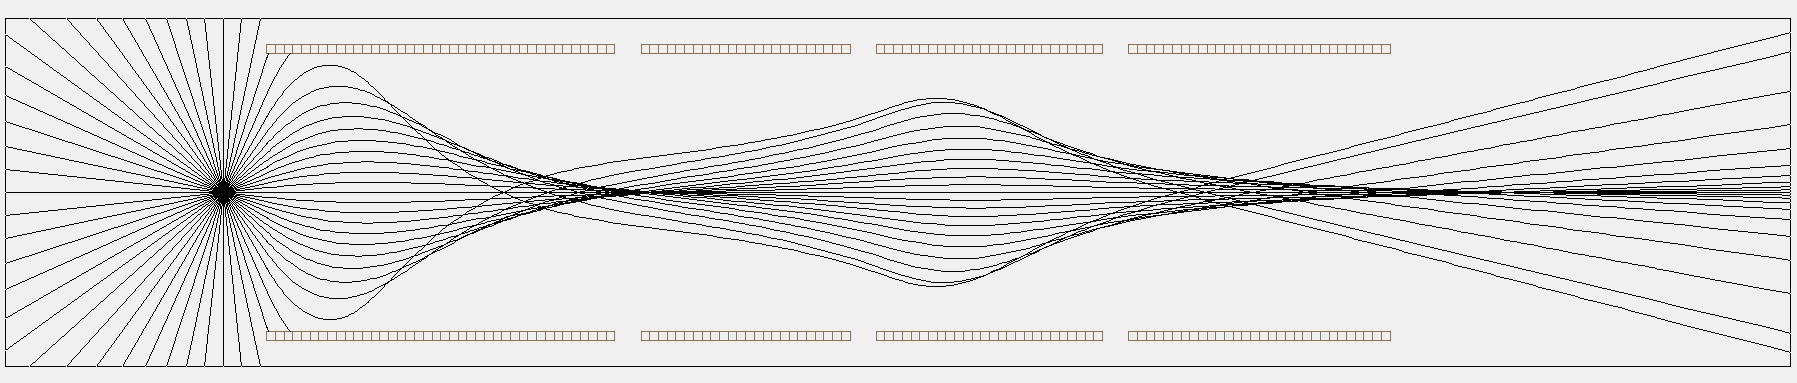
\includegraphics[width = 366 pt]{Figure/05/2a.jpg}
\caption{Caption.}
\label{05simulaceVlastniDelo}
\end{figure}

Konfiguraci lze ještě vylepšit jednoduše tím, že se wolframové vlákno umístí dovnitř první elektrody, jak ukazuje simulace na Obr. DOPLN., kde je zdroj elektronů umístěný 1 cm od levého kraje první elektrody. Nastavení simulace je jinak stejné jako u té předchozí, napětí na poslední elektrodě je ovšem $U_4 = 18$~kV, což se více blíží napětí, kterého jsme byli schopni dosáhnout bez probíjení. I tak se dalo očekávat, že alespoň na stínítku bychom mohli pozorovat stopu svazku. Nicméně ani s jednou konfigurací jsme ve vakuové komoře nakonec neuspěli. Další postup proto zahrnoval použítí zakoupeného průmyslového děla.\\

\begin{figure}[htbp!]
\centering
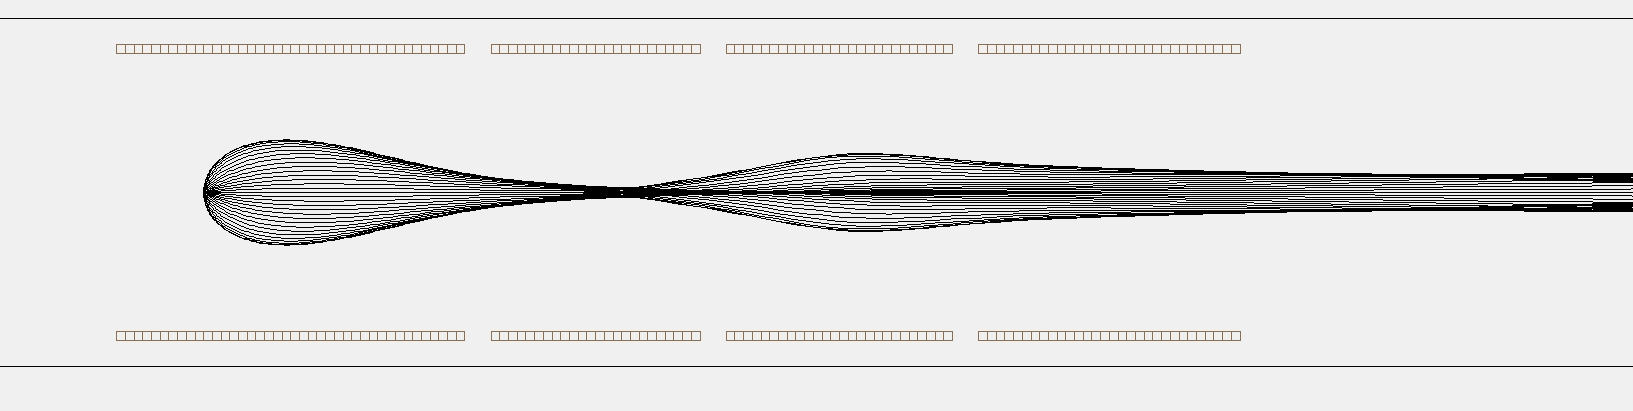
\includegraphics[width = 366 pt]{Figure/05/2c.jpg}
\caption{Caption.}
\label{05simulaceVlastniDeloWehnelt}
\end{figure}

\section{Urychlování svazku z průmyslového děla}

Zakoupené elektronové dělo bylo od výroby dostatečně dobře fokusované. Nejmenší možný průměr svazku uvedený výrobcem byl $d = 120$~$\mu$m ve vzdálenosti $l = 56$~mm. Proto fokusační soustava ztrácela svůj význam. Přesto však bylo třeba pro účely detekce svazek urychlit. Maximální energie svazku byla totiž $E = 5$~keV. Nakonec i možnost posouvat ohnisko svazku a tak jej fokusovat nebo defokusovat nezávisle na nastavení na průmylsovém děle se jevila jako zajímavá. Proto se finální fokusovací soustava skládala opět ze čtyř elektrod.\\

Elektrody byly tentokrát umístěny ve větší vzdálenosti od sebe, abychom omezili pravděpodobnost probíjení mezi nimy, ačkoliv jsme zcela s jistotou nevěděli, zdali k němu docházelo. Svazek z děla je v následujích simulacích reprezentován rovnoběžnými trajektoriemi dvou elektronů, které jej hypoteticky ohraničují. Průměr svazku je $d = 1$ mm a energie $E = 5$ keV. Ostatní parametry finální konfigurace jsou následující:
\begin{itemize}
	\item Vzdálenost mezi elektrodami: $\Delta x = 2$~mm
	\item Geometrie elektrod: $d = 30$~mm, $l_0 = 40$ mm, $l_1 = 24$ mm, $l_2 = 26$ mm, $l_3 = 30$ mm
	\item Napětí na elektrodách:
	\begin{enumerate}
		\item $U_1 = 1$ kV, $U_2 = 5$ kV, $U_3 = 1$ kV, $U_4 = 18$ kV
		\item $U_1 = 1$ kV, $U_2 = 15$ kV, $U_3 = 1$ kV, $U_4 = 18$ kV
		\item $U_1 = 1$ kV, $U_2 = 1$ kV, $U_3 = 1$ kV, $U_4 = 18$ kV
	\end{enumerate}
\end{itemize}

Ačkoliv to není z Obr. \ref{05simulaceFinalniKonfigurace} vzhledem k nepoměru mezi průměry svazku a elektrod zcela patrné, simulace ukazuje, že nastavováním napětí na druhé elektrodě lze teoreticky posouvat ohnisko, tudíž bychom mohli na stínítku pozorovat zvětšování, popř. zmenšování profilu svazku. Pro napětí $U_2 = 5$~kV se ohnisko nachází přibližně ve vzdálenosti $x = 178$ mm od levého kraje první elektrody. Pro napětí $U_2 = 15$~kV je to $x = 112$~mm a pro $U_2 = 1$~kV je $x = 204$~mm. Takový posun by se měl na stínítku v pevné vzdálenosti od zdroje projevit změnou průměru profilu řádově až v milimetrech, což by měl být pozorovatelný jev.\\

\begin{figure}[htbp!]
\centering
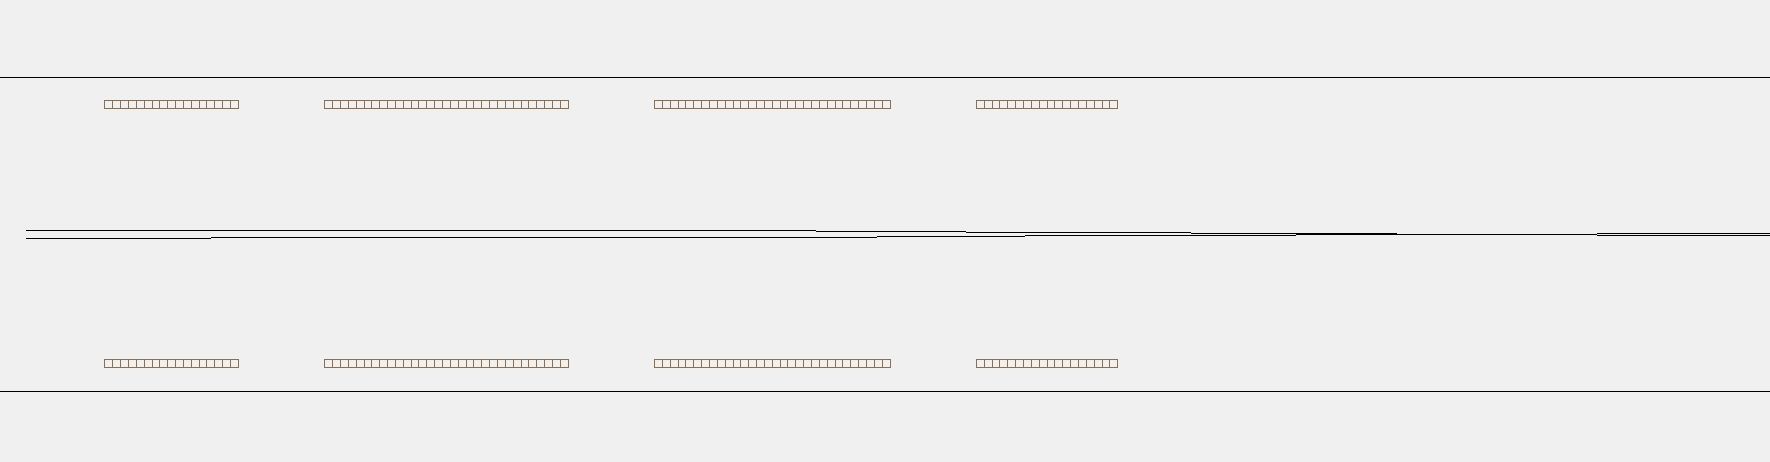
\includegraphics[width = 366 pt]{Figure/05/1a.jpg}
\vfill
\vfill
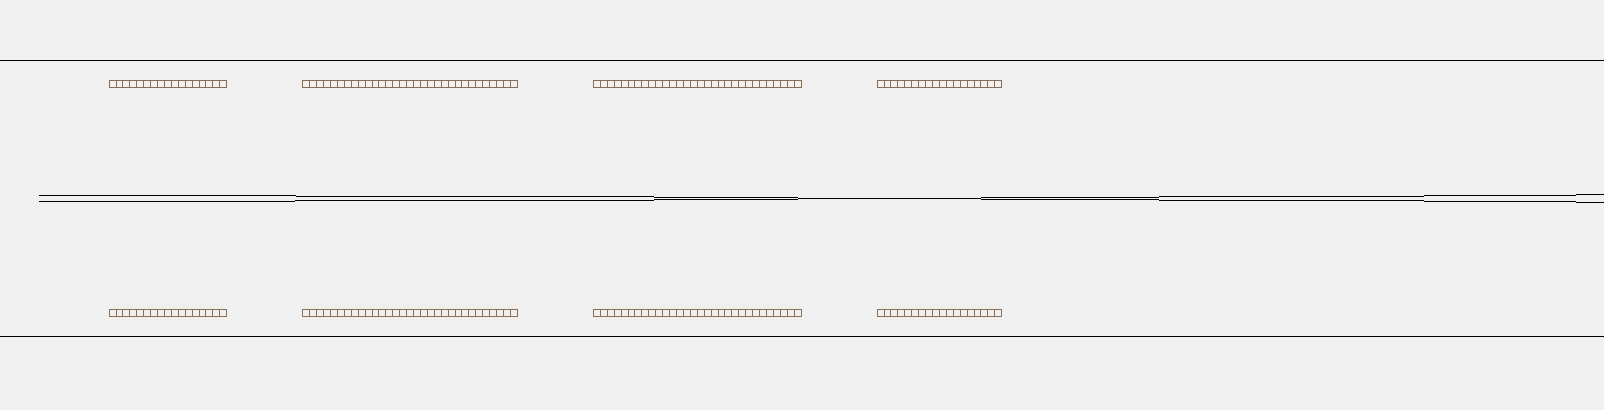
\includegraphics[width = 366 pt]{Figure/05/1b.jpg}
\vfill
\vfill
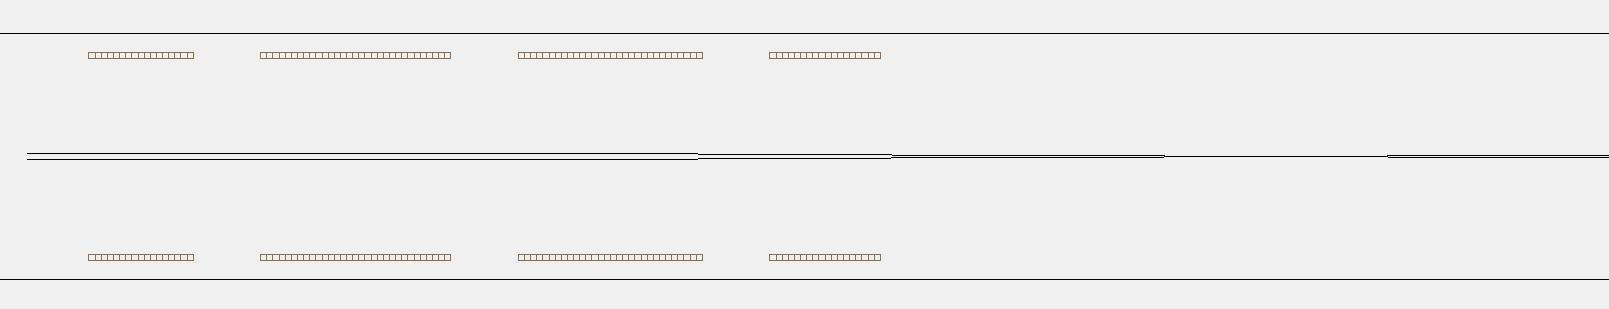
\includegraphics[width = 366 pt]{Figure/05/1c.jpg}
\caption{Caption.}
\label{05simulaceFinalniKonfigurace}
\end{figure}

\section{Zkouška děla se stínítkem}

\section{Závěr}
